\documentclass[10pt]{beamer}
\usepackage{preamble}
\usetheme{metropolis}
\usepackage{appendixnumberbeamer}
\usepackage{animate}
\title{Getting Started with \text{\LaTeX}}
\subtitle{And why I don't use Word anymore}
\date{\today}
\author{Jack Naylor}
\institute{Treasurer - PhySoc, University of Sydney}
\titlegraphic{\hfill
\includegraphics[height=2cm]{reclogo.png}\flushright
\includegraphics[height=1cm]{aiaa-logo-blue.png}}
\begin{document}

\maketitle
\section{What is \text{\LaTeX}?}
\begin{frame}{A bit of Background}
    
\end{frame}
\begin{frame}
\centering
Something to keep in mind throughout this presentation: \emph{\alert{every single slide} is done in \LaTeX}
\end{frame}
\section{What can I do?}
\begin{frame}
\centering
    In short: anything you can do with Word + much much more!!
\end{frame}
\begin{frame}{Images}
    
\end{frame}
\begin{frame}
    \begin{figure}
        \centering
        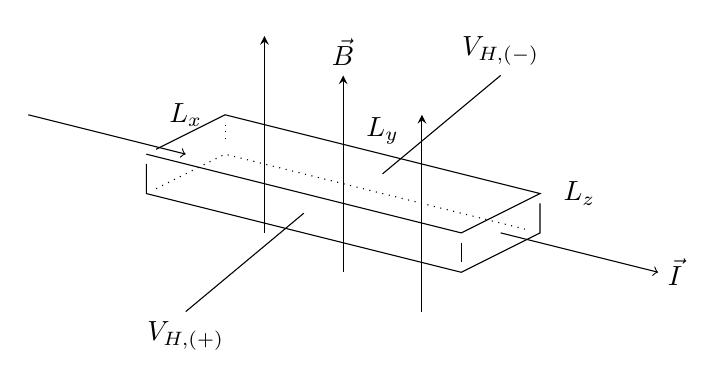
\begin{tikzpicture}
\draw (-1.5,2) node (v1) {} -- (2.5,1) node (v7) {} -- (3.5,1.5) node (v2) {} -- (-0.5,2.5) node (v5) {} -- (v1) -- (-1.5,1.5) node (v3) {} -- (2.5,0.5) node (v8) {} -- (3.5,1) node (v4) {} -- (v2);
\node[above] (v9) at (1.5,2) {$L_y$};
\node at (4,1.5) {$L_z$};
\node at (-1,2.5) {$L_x$};
\draw[->] (3,1) -- (5,0.5);
\draw[<-] (-1,2) -- (-3,2.5);
\draw[dotted] (v3) -- (-0.5,2) node (v6) {} -- (v4);
\draw[dotted] (v5) -- (v6);
\draw (v7) -- (v8);
\draw (0.5,1.25) -- (-1,0);
\draw (1.5,1.75) -- (3,3);
\node[below] at (-1,0) {$V_{H,(+)}$};
\node[above] at (3,3) {$V_{H,(-)}$};
\node[right] at (5,0.5) {$\vec{I}$};
\draw[-stealth] (0,1) -- (0,3.5);
\draw[-stealth] (1,0.5) -- (1,3);
\draw[-stealth] (2,0) -- (2,2.5);
\node[above] at (1,3) {$\vec{B}$};
\end{tikzpicture}
\caption{Semiconductor sample in $B$ field}

    \end{figure}
\end{frame}
\begin{frame}
    \begin{figure}
\animategraphics[loop,autoplay,scale=0.5]{5}{elon-gif/new_}{0}{449}
\caption{Gif of NACA3512 turbine in wind tunnel}
\end{figure}
\end{frame}
\begin{frame}
    
\end{frame}
\begin{frame}{Maths}
\begin{itemize}
    \item Inline:\\
    It is known that $y=x^2+2x+4$ is a parabola.\par
    \item Block:\\
    Here is a Fourier transform:
    \[\mathcal{F}\left(\omega\right)=\int_{-\infty}^\infty f(t) e^{i\omega t}\dd t\]
    \item Numbered:
    \begin{subequations}
    \begin{align}
        \ket{+_x} &= \frac{1}{\sqrt{2}} \ket{+} + \frac{1}{\sqrt{2}} \ket{-}\\
        \ket{-_x} &= -\frac{1}{\sqrt{2}} \ket{+} + \frac{1}{\sqrt{2}} \ket{-}\\
        \abs{\braket{+}{+_x}}^2 &= 0.5
    \end{align}
    \end{subequations}
\end{itemize}


\end{frame}
\begin{frame}{Plots}
    
\end{frame}
\end{document}
